\begin{frame}
	\frametitle{Time Hierarchy}
	\framesubtitle{Vorraussetzungen}
	Wiederholung :
	\begin{itemize}[<+->]
		\item Für $i\in \mathbb{N}$ beschreibt i die TM $M_i$
		\item Jede TM wird von unendlich vielen $i\in \mathbb{N}$ beschrieben
		\item Es existiert eine universelle TM U, die jede TM mit logarithmischem Overhead 					simulieren kann
	\end{itemize}
\end{frame}
\begin{frame}
	\frametitle{Time Hierarchy}
	\framesubtitle{Vorraussetzungen}
	\begin{KITexampleblock}{Universelle TM}
	TM $M_i$ läuft bei Eingabe x in $\mathcal{O}(f(n))$
	$\Rightarrow$ TM U läuft bei Eingabe i, x in $\mathcal{O}(f(n)log(f(n)))$
	\end{KITexampleblock}
\end{frame}
\begin{frame}
	\frametitle{Time Hierarchy}
	\framesubtitle{Vorraussetzungen}
	\begin{KITinfoblock}{Definition Time-constructible functions}
		Wir nennen eine Funktion f time-constructible, falls gilt : \newline
		f(n) ist in $\mathcal{O}(f(n))$ berechenbar. 
	\end{KITinfoblock}
	
	\bigskip
	\pause	
	
	\begin{KITinfoblock}{Definition \DTIME }
		\DTIME(f(n)) = $\lbrace$ L $\vert \exists$ deterministische Turingmaschine ,
		 die L in $\mathcal{O}(f(n))$ entscheidet $\rbrace$
	\end{KITinfoblock}
\end{frame}
\begin{frame}
	\frametitle{Time Hierarchy}
	\framesubtitle{Deterministische Time Hierarchy}
	
	\begin{KITinfoblock}{Satz: Time Hierarchy Theorem, 65}
	Seien $f, g$  time-constructible mit  
	$f(n)\log(f(n)) \in o(g(n))$ , dann gilt
	$\DTIME(f(n)) \subsetneq \DTIME(g(n))$
		
	\end{KITinfoblock}
	\bigskip
	\begin{columns}
	\column{.5\textwidth}
	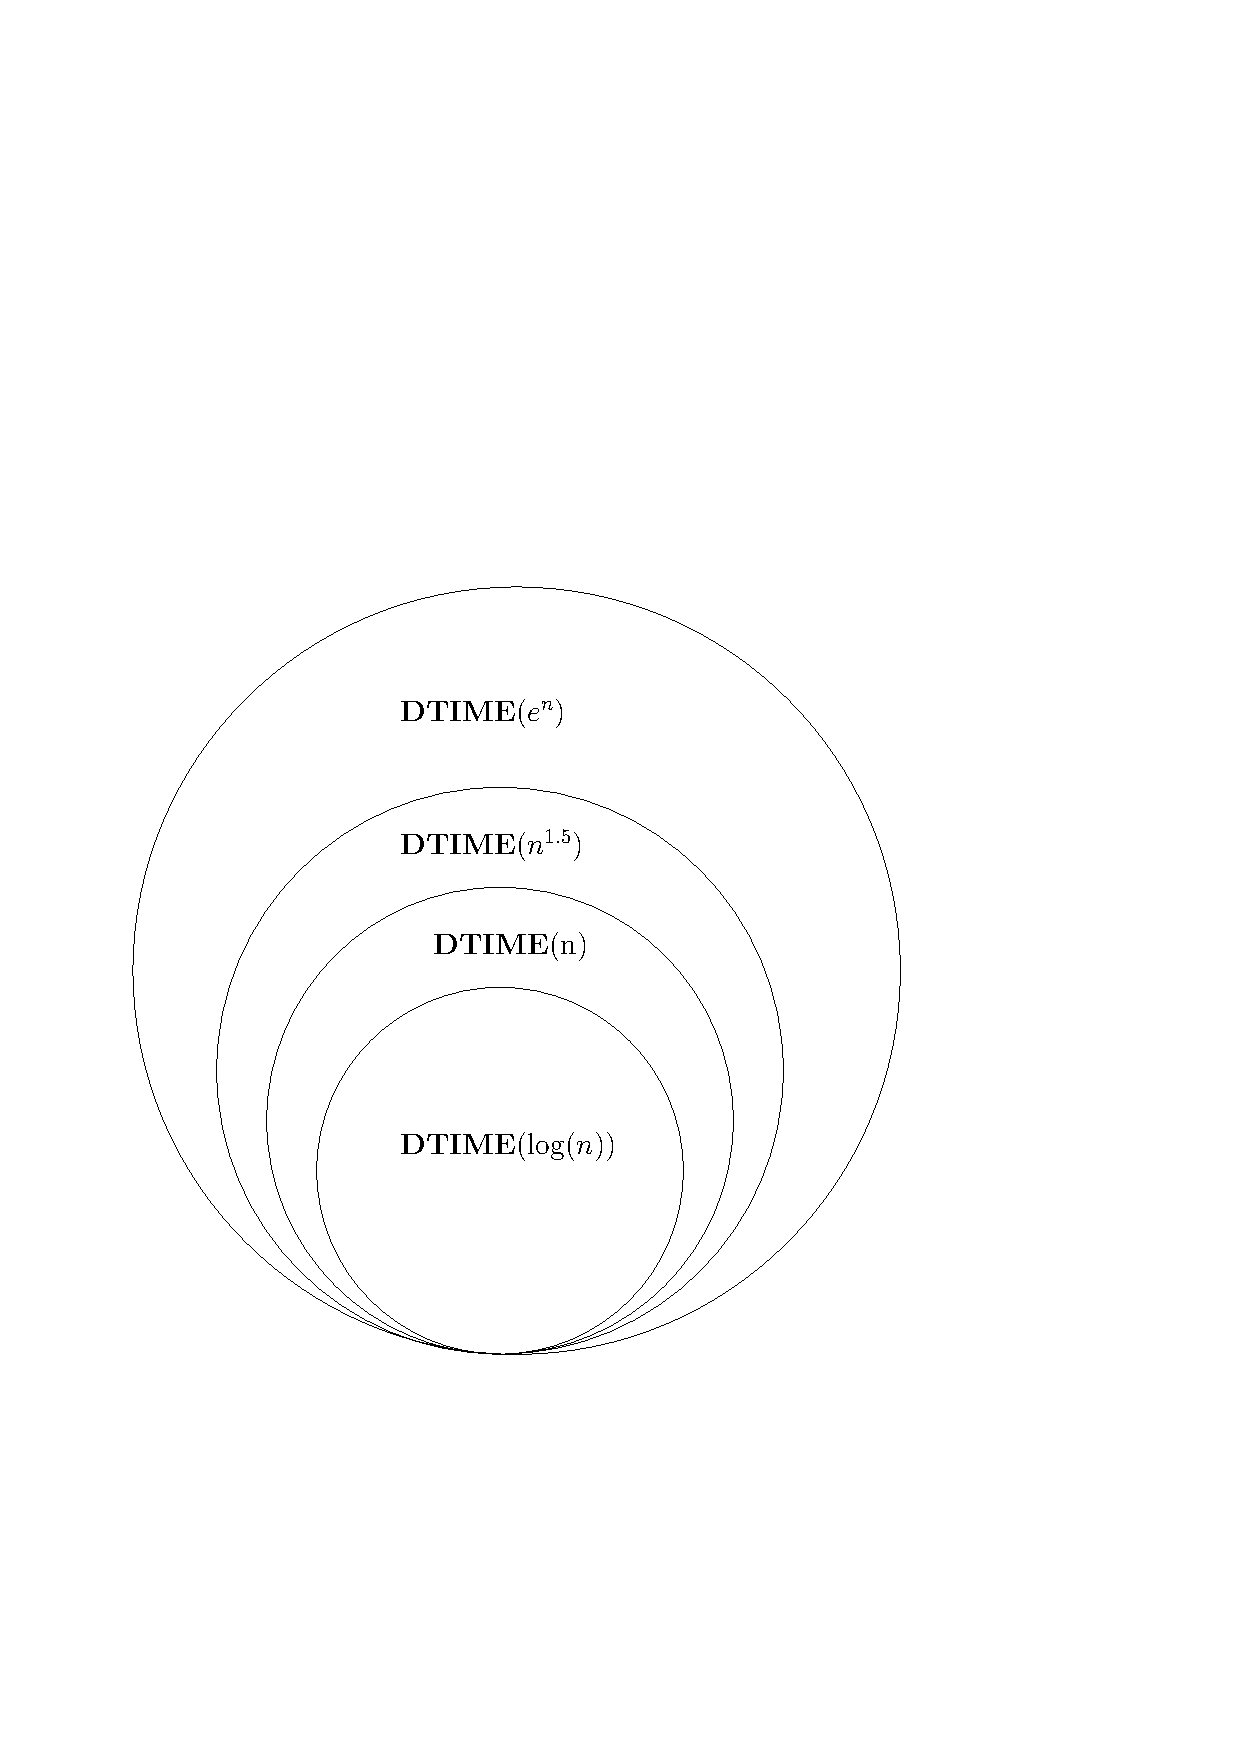
\includegraphics[scale=0.3]{images/timehierarchy.pdf}
		
	\pause
	\column{.5\textwidth}
	Frage : Warum brauchen wir den Faktor $\log(f(n))$ ?
	\end{columns}
\end{frame}

\begin{frame}
	\frametitle{Time Hierarchy}
	\framesubtitle{{Beweis det. Time Hierarchy}}
	Wir zeigen $\DTIME(n) \subsetneq \DTIME(n^{1.5})$
	\bigskip
	\pause
	\begin{KITinfoblock}{Definition Turing Maschine D} 
		Bei Eingabe $x$ : Simuliere die TM $M_x$ mit Eingabe $x$ genau für $|x|^{1.4}$
		 						Schritte. Danach gebe folgendes aus :
		\begin{equation*}
		D(x) = 
		\begin{cases}
			\overline{M_x(x)} & \text{falls die Simulation eine Ausgabe hatte} \\
			0 & \text{sonst}
			
		\end{cases}
		\end{equation*}			
		\bigskip
		Sei $L =  \lbrace x \vert D(x) = 1  \rbrace$ die von $D$ erzeugte Sprache
	\end{KITinfoblock}
\end{frame}

\begin{frame}
	\frametitle{Time Hierarchy}
	\framesubtitle{Beweis det. Time Hierarchy}
	\begin{KITblock}{Behauptung}
		$L \in \DTIME(n^{1.5})$ und $L \notin \DTIME(n)$
	\end{KITblock}
	\pause
	\begin{itemize}[<+->]
		\item Wir nehmen an , dass $L \in \DTIME(n)$
		\item $\Rightarrow \exists$ Turing Maschine $M$ , die $L$ entscheidet \newline
		($\Leftrightarrow \forall x \in {\lbrace 0,1 \rbrace }^{*}$ D(x) = M(x)) und
		für Eingabe x höchstens c|x| Schritte benötigt. (c ist konstant)
		\item Wir konstruieren Wiederspruch , indem wir $D$ eine Gödelnummer $x$ mit
			$M_x = M$ als Eingabe geben.
	\end{itemize}
\end{frame}

\begin{frame}
	\frametitle{Time Hierarchy}
	\framesubtitle{Beweis det. Time Hierarchy}
	\begin{KITinfoblock}{Definition Turing Maschine D} 
		Bei Eingabe $x$ : Simuliere die TM $M_x$ mit Eingabe $x$ genau für $|x|^{1.4}$
		 Schritte. Danach gebe das invertierte Ergebniss von $M_x$	aus			
	\end{KITinfoblock}
	
	\begin{itemize}[<+->]
		\item Wollen $|x|$ groß genug, dass D für $M_x$ eine Ausgabe erhält !
		\item M simuliert auf U läuft in $c|x|\log(|x|)$
		\item Wir wählen dazu Gödelnummer $x$ mit $M_x = M$ so groß, dass gilt :
			$|x|^{1.4} > c|x|\log(|x|)$		
		\item Damit läuft $M_x$ in der Simulation in D komplett durch und D invertiert
			das Ergebniss
		\item Nun gilt $D(x) \neq M(x)$ 	\qed 
		\item Beweis ähnlich auf allgemeinen Fall übertragbar
	\end{itemize}
\end{frame}
